% !TeX root = main.tex

\section{实验结果}

\subsection{未抛光}

\subsubsection{粉煤灰: 0\%}

\begin{figure}
  \centering
  \subcaptionbox{2000x}{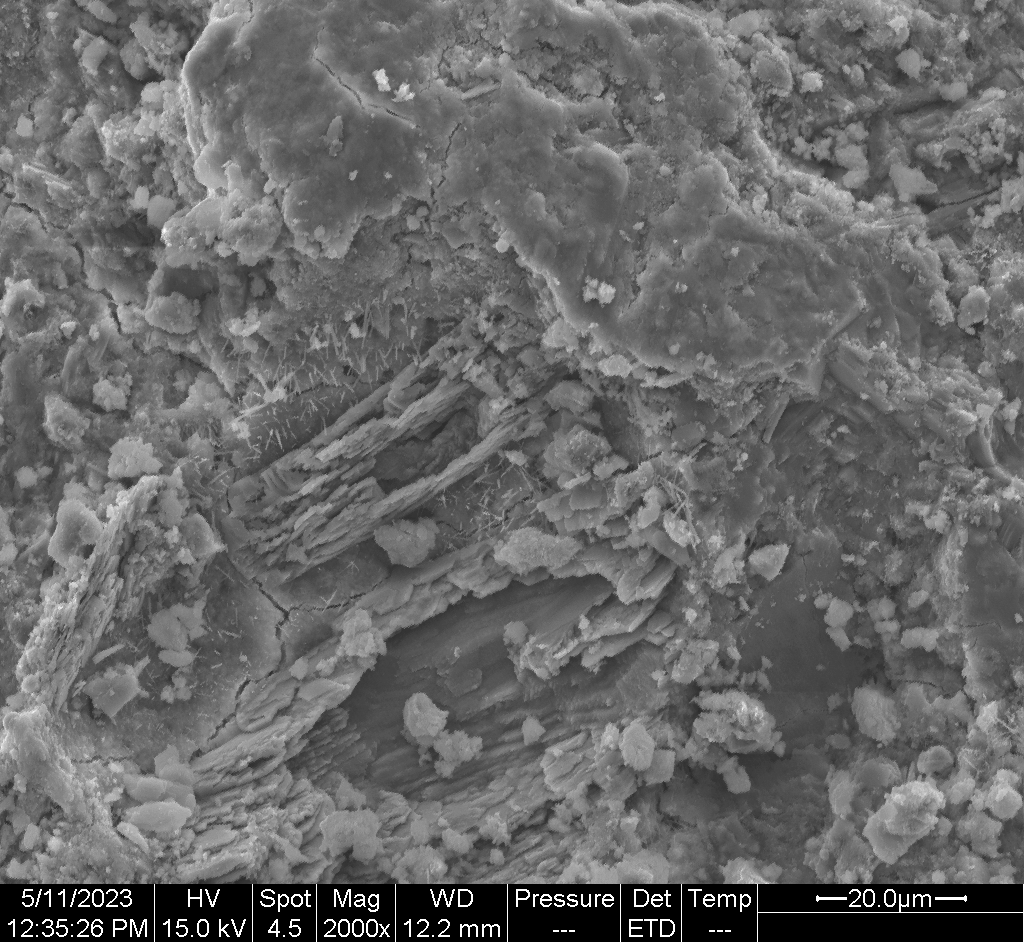
\includegraphics[height = 0.28 \linewidth]{assets/00-unpolished-02000x-ETD.png}} \quad
  \subcaptionbox{5000x}{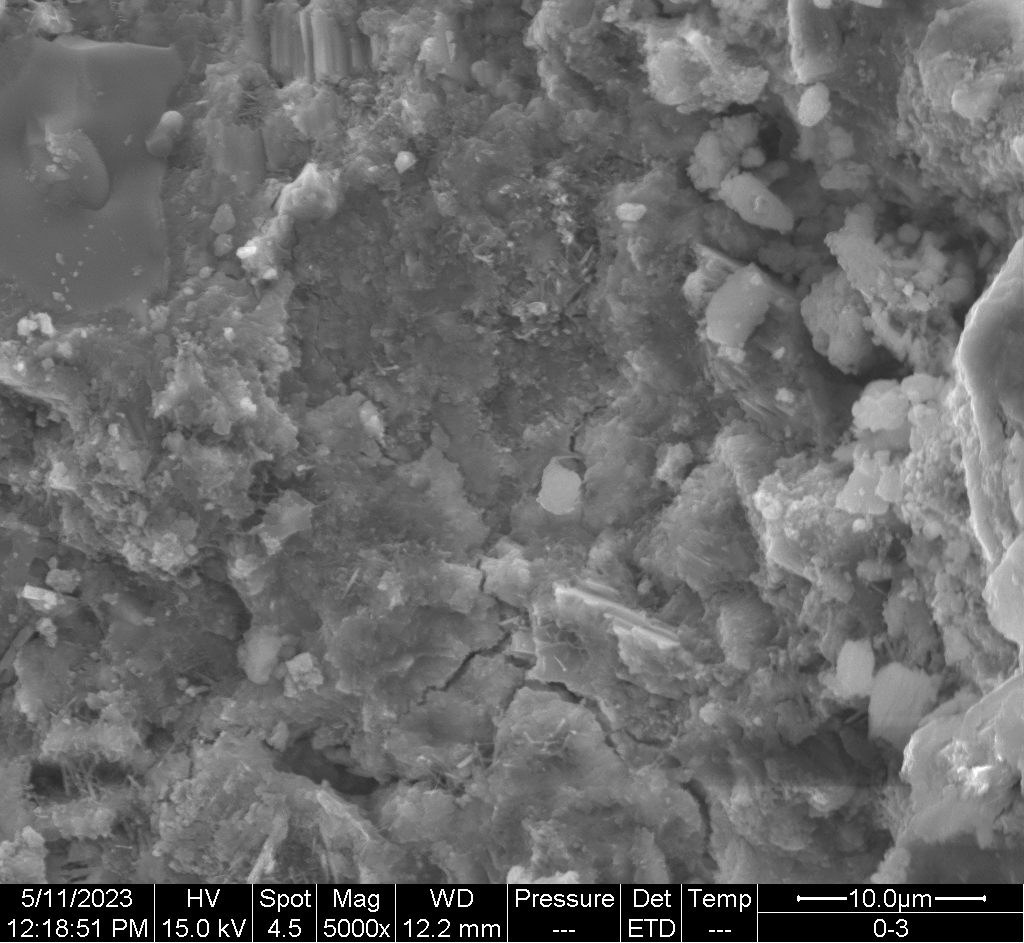
\includegraphics[height = 0.28 \linewidth]{assets/00-unpolished-05000x-ETD.png}} \quad
  \subcaptionbox{10000x}{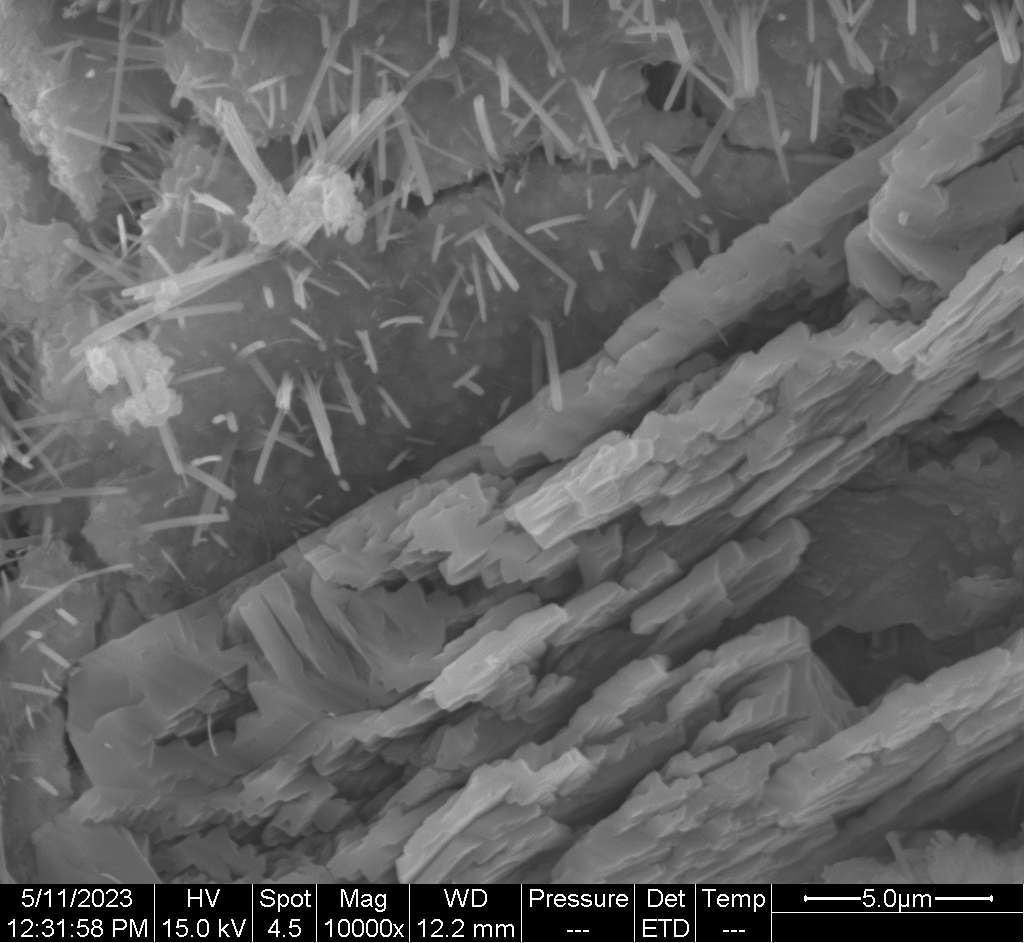
\includegraphics[height = 0.28 \linewidth]{assets/00-unpolished-10000x-ETD.png}}
  \caption{ETD}
\end{figure}

\subsubsection{粉煤灰: 15\%}

\begin{figure}
  \centering
  \subcaptionbox{1000x}{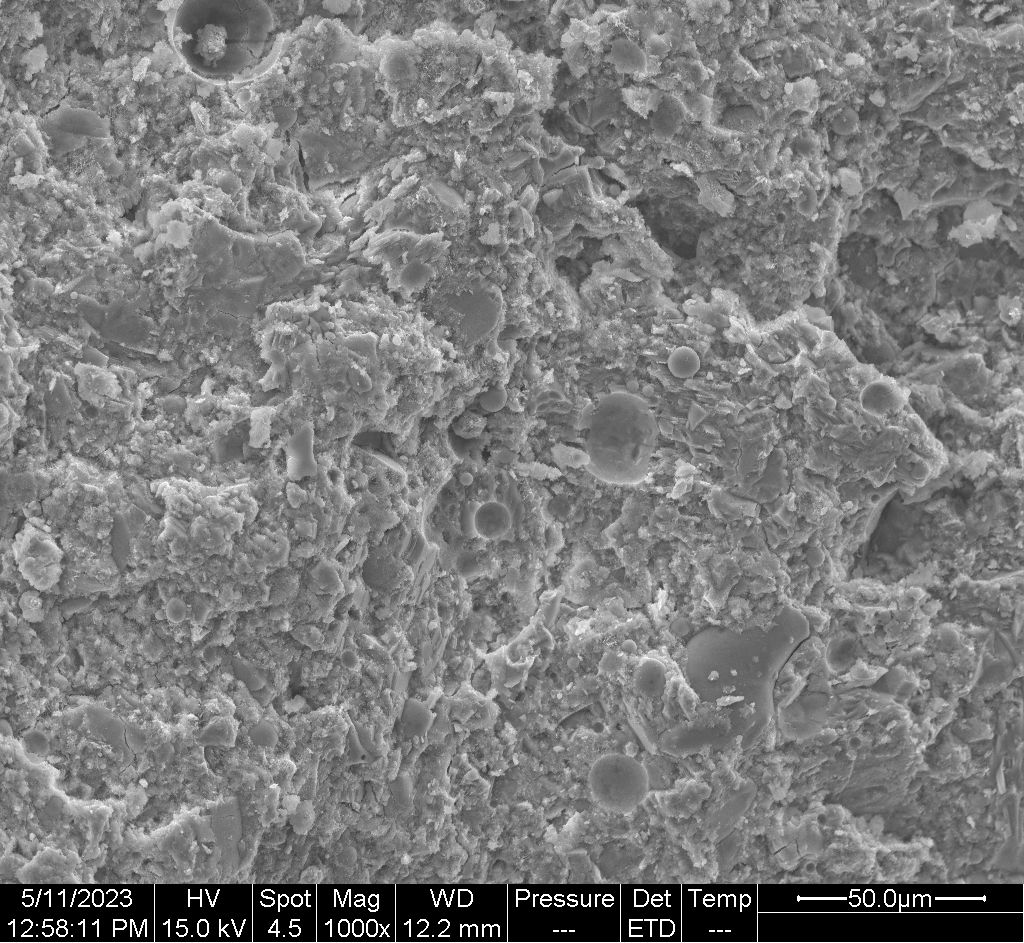
\includegraphics[height = 0.21 \linewidth]{assets/15-unpolished-01000x-ETD.png}} \quad
  \subcaptionbox{4000x}{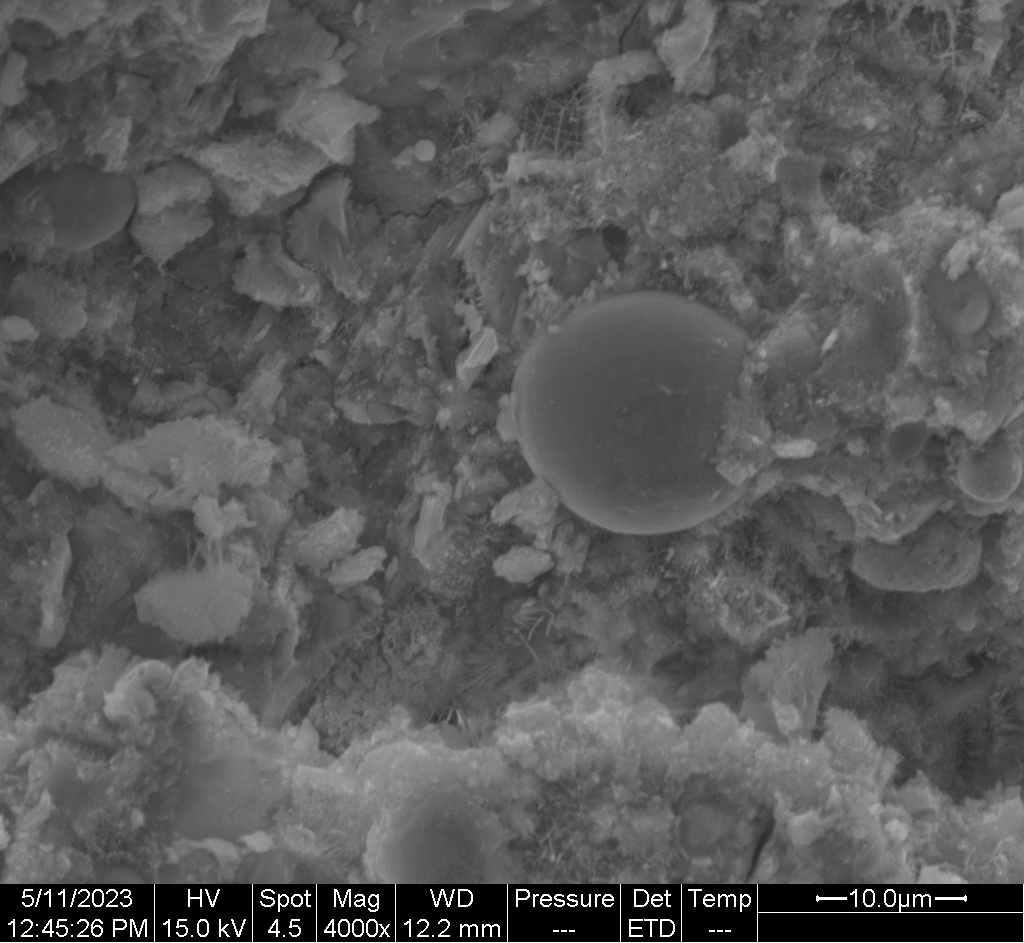
\includegraphics[height = 0.21 \linewidth]{assets/15-unpolished-04000x-ETD.png}} \quad
  \subcaptionbox{10000x}{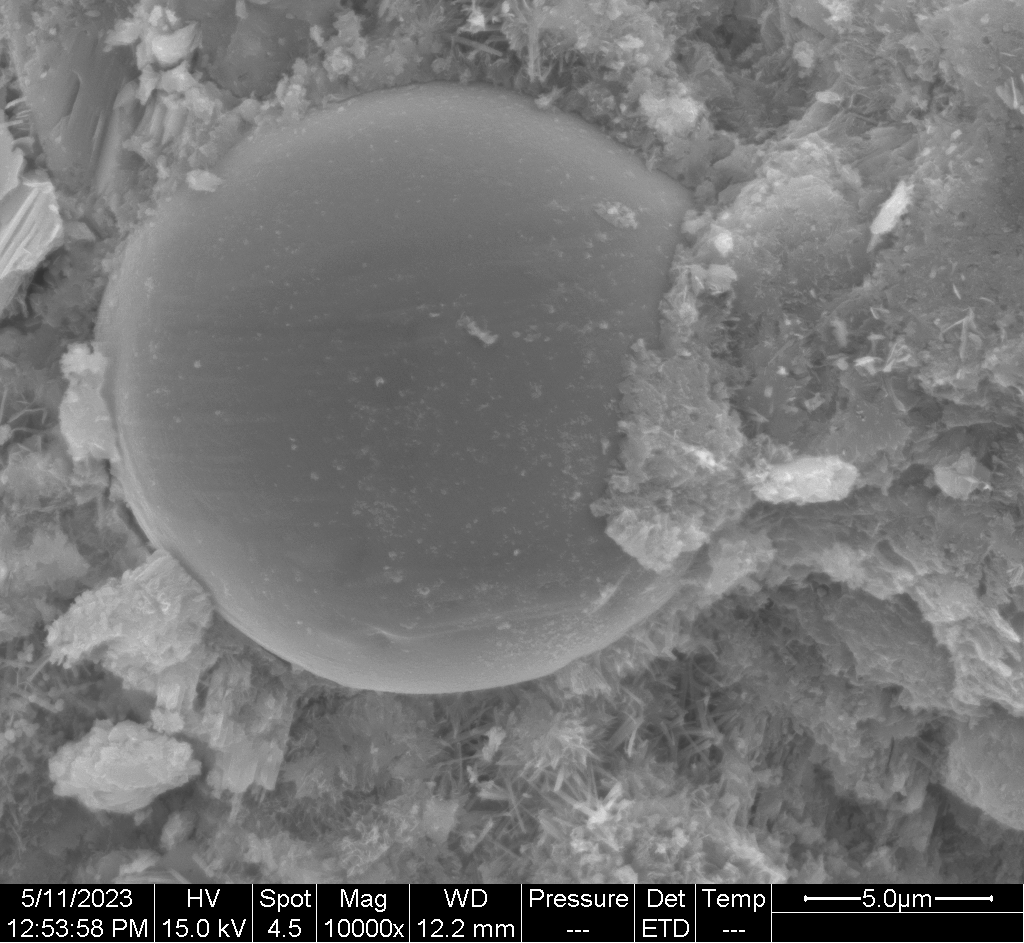
\includegraphics[height = 0.21 \linewidth]{assets/15-unpolished-10000x-ETD.png}} \quad
  \subcaptionbox{20000x}{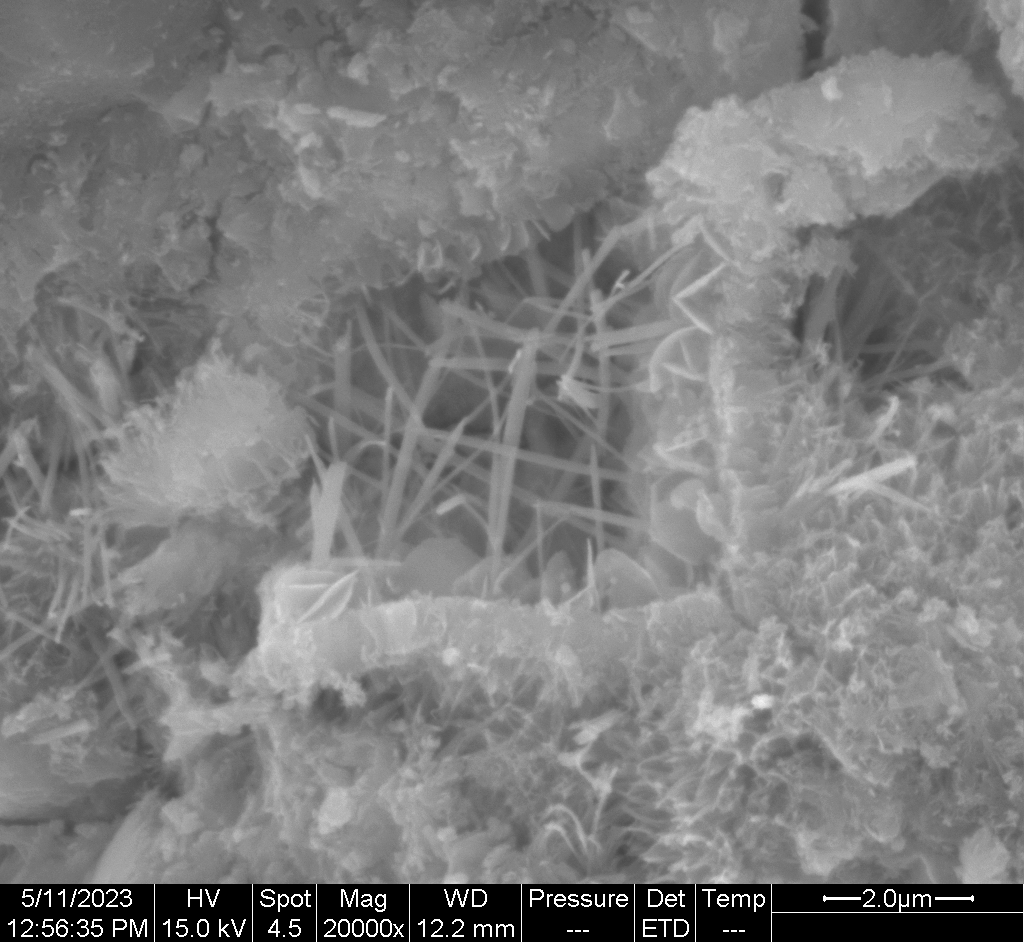
\includegraphics[height = 0.21 \linewidth]{assets/15-unpolished-20000x-ETD.png}}
  \caption{ETD}
\end{figure}

\subsubsection{粉煤灰: 30\%}

\begin{figure}
  \centering
  \subcaptionbox{1000x}{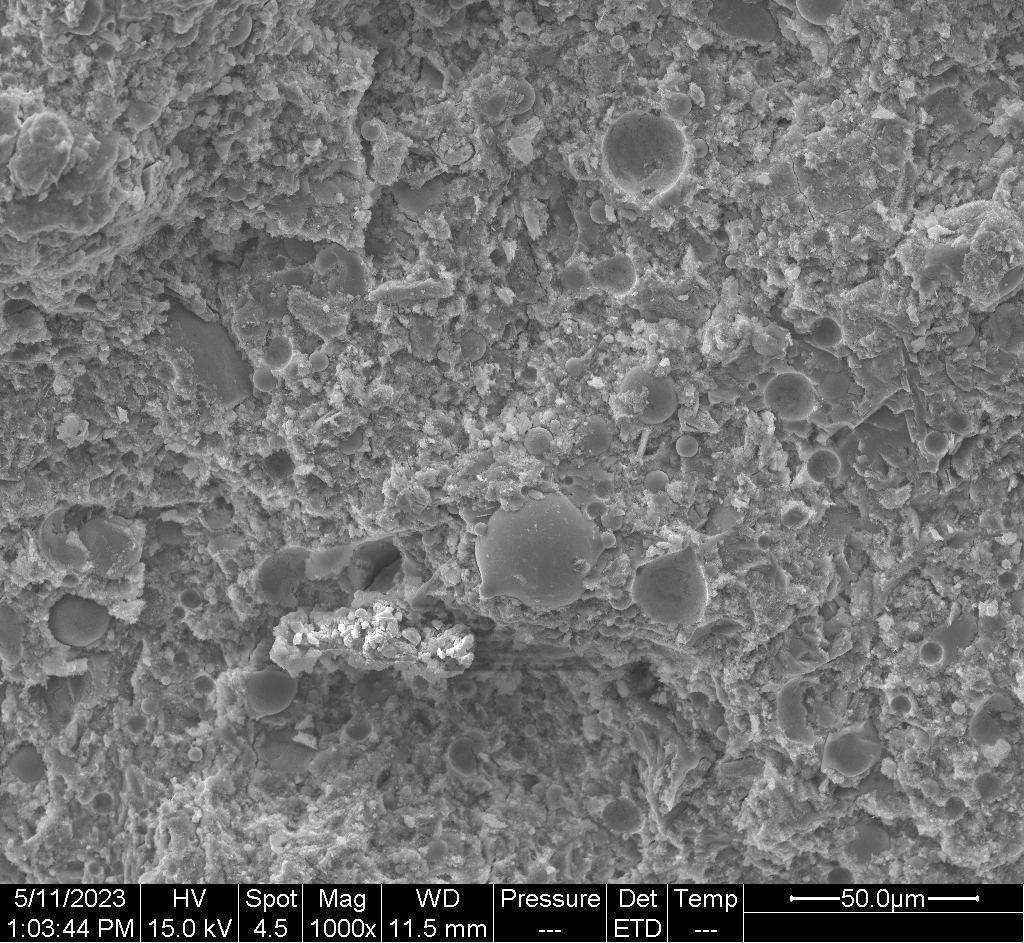
\includegraphics[height = 0.28 \linewidth]{assets/30-unpolished-01000x-ETD.png}} \quad
  \subcaptionbox{3000x}{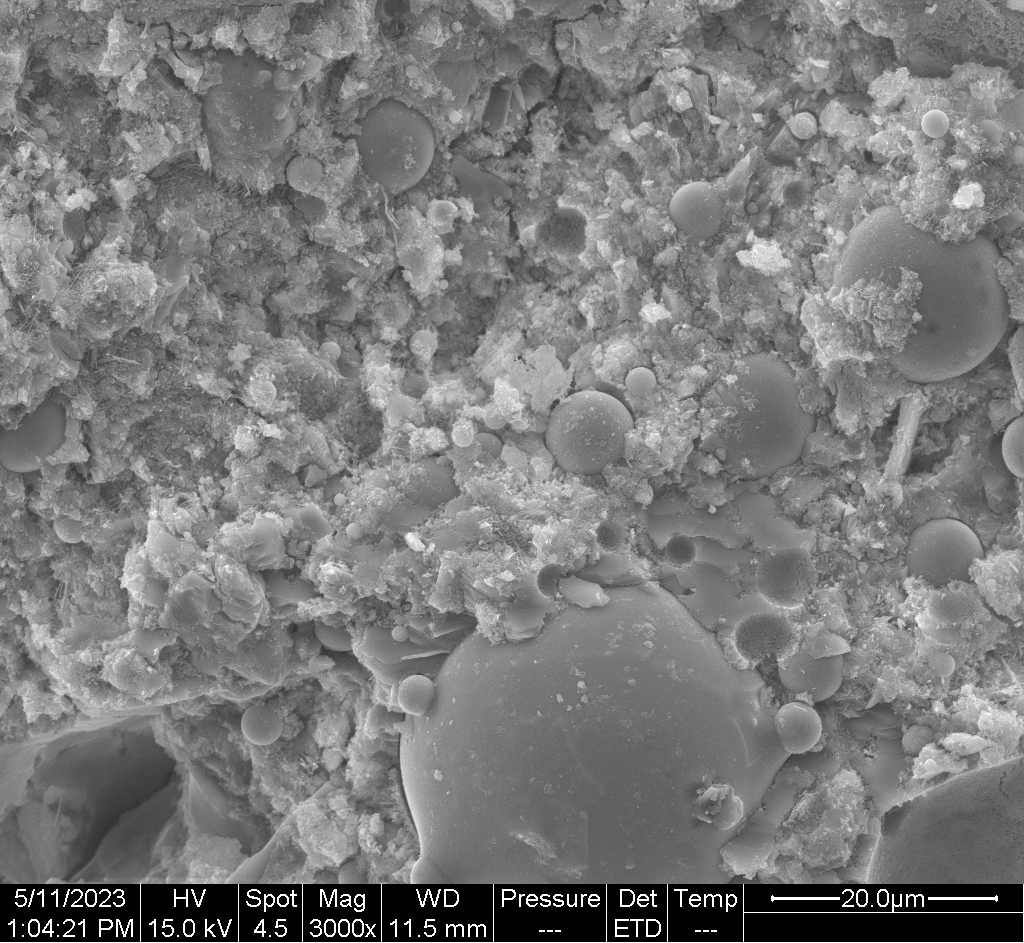
\includegraphics[height = 0.28 \linewidth]{assets/30-unpolished-03000x-ETD.png}} \quad
  \subcaptionbox{10000x}{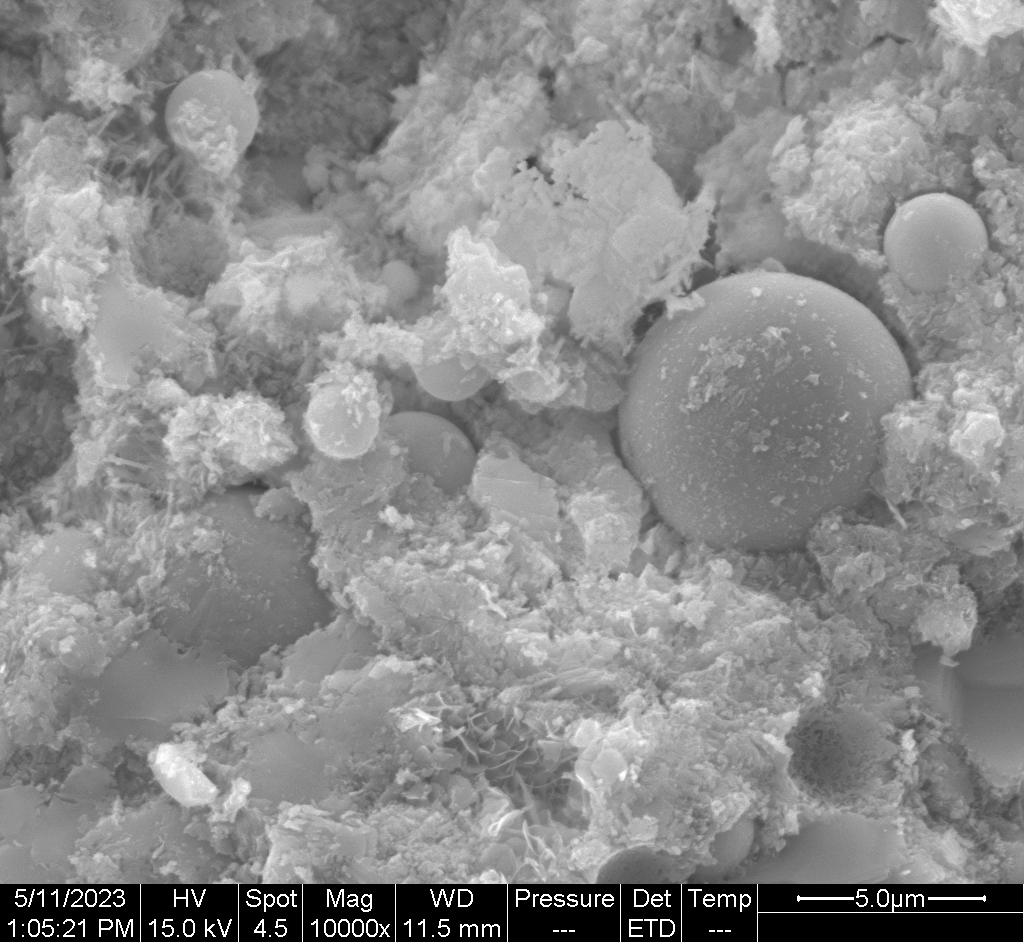
\includegraphics[height = 0.28 \linewidth]{assets/30-unpolished-10000x-ETD.png}}
  \par \vspace{1em}
  \subcaptionbox{30000x}{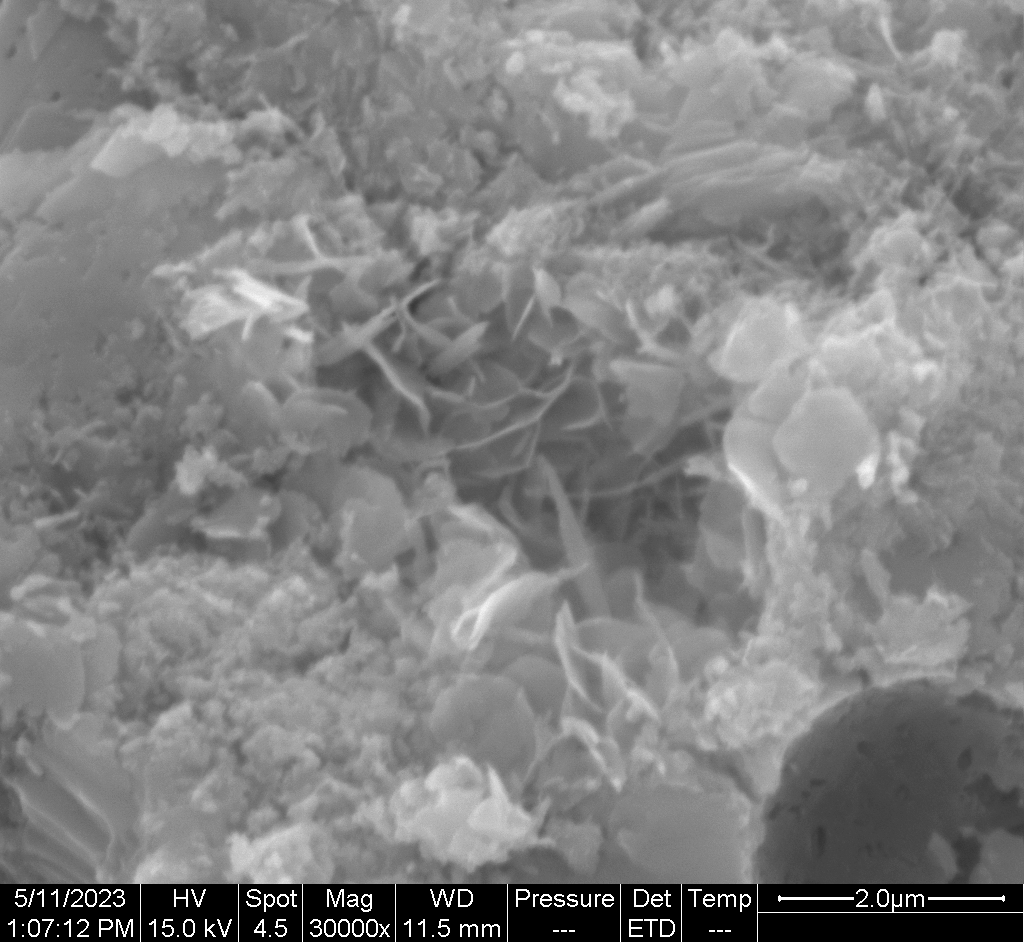
\includegraphics[height = 0.28 \linewidth]{assets/30-unpolished-30000x-ETD.png}} \quad
  \subcaptionbox{60000x}{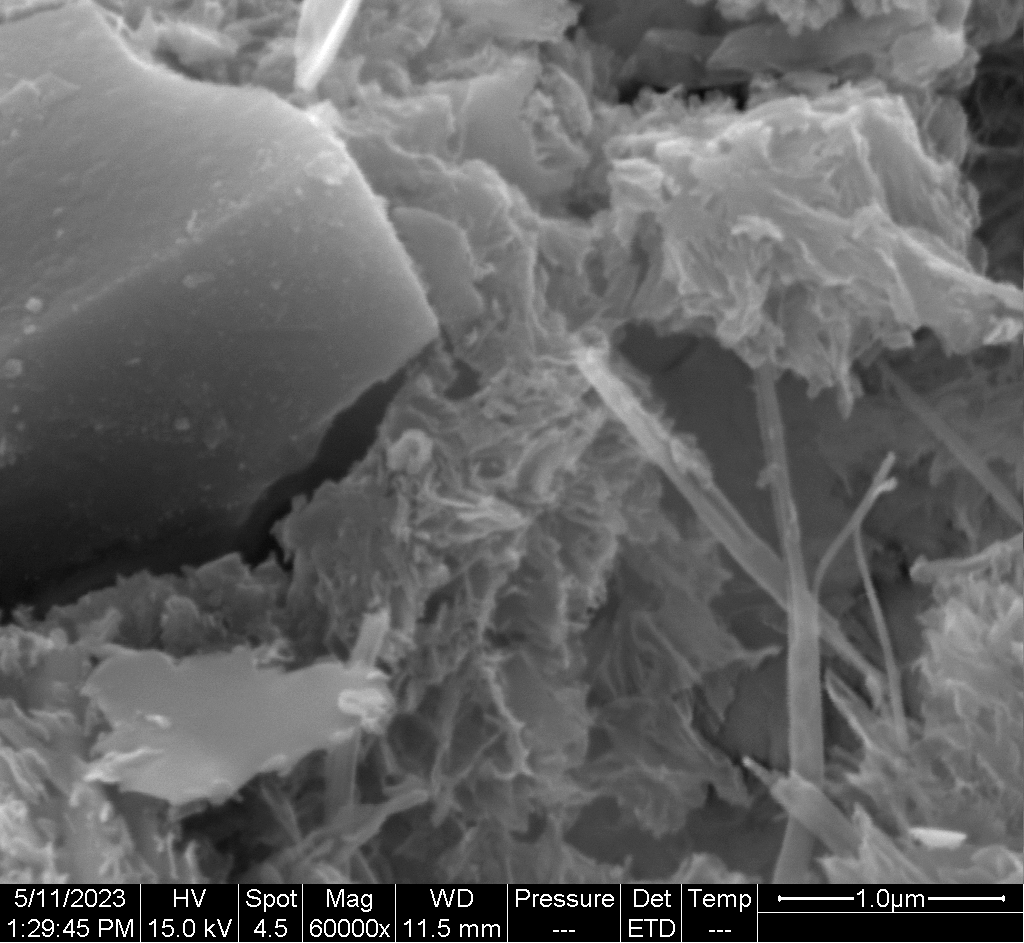
\includegraphics[height = 0.28 \linewidth]{assets/30-unpolished-60000x-ETD.png}}
  \caption{ETD}
\end{figure}

\subsection{抛光}

\subsubsection{粉煤灰: 0\%}

\begin{figure}
  \centering
  \subcaptionbox{500x}{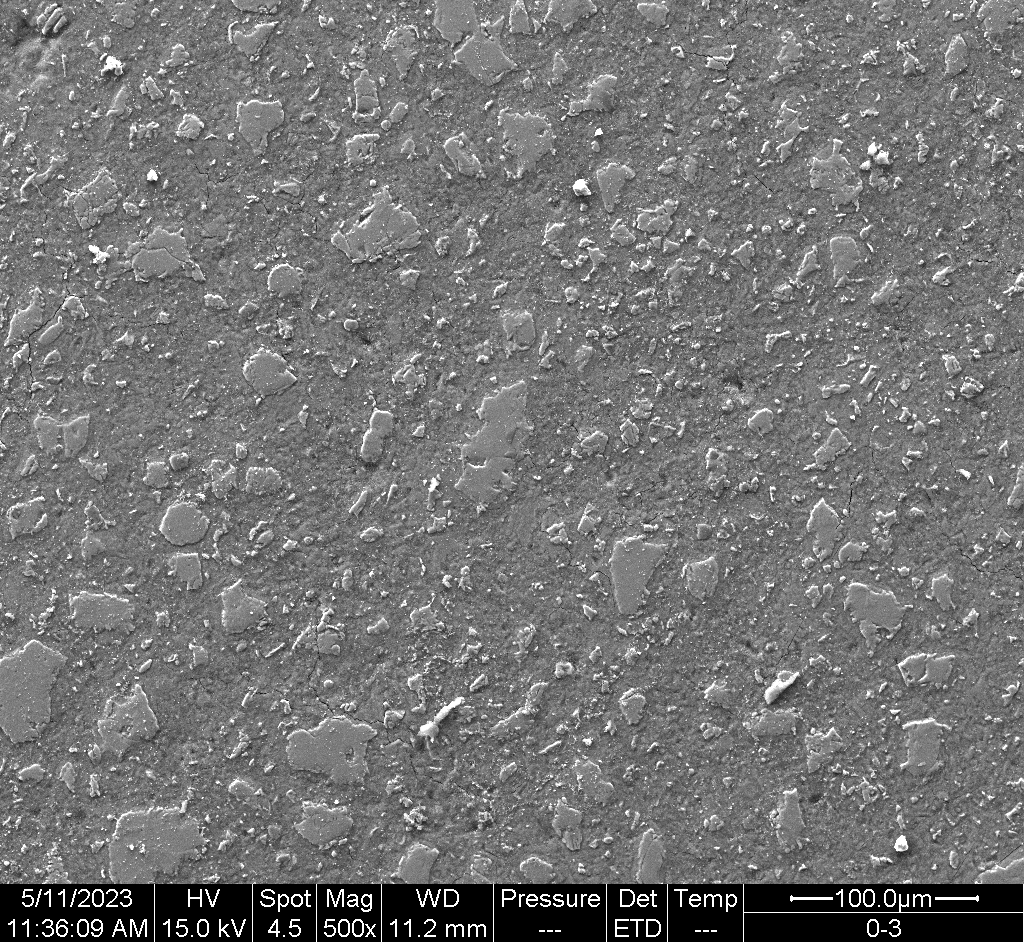
\includegraphics[height = 0.21 \linewidth]{assets/00-polished-00500x-ETD.png}} \quad
  \subcaptionbox{2000x}{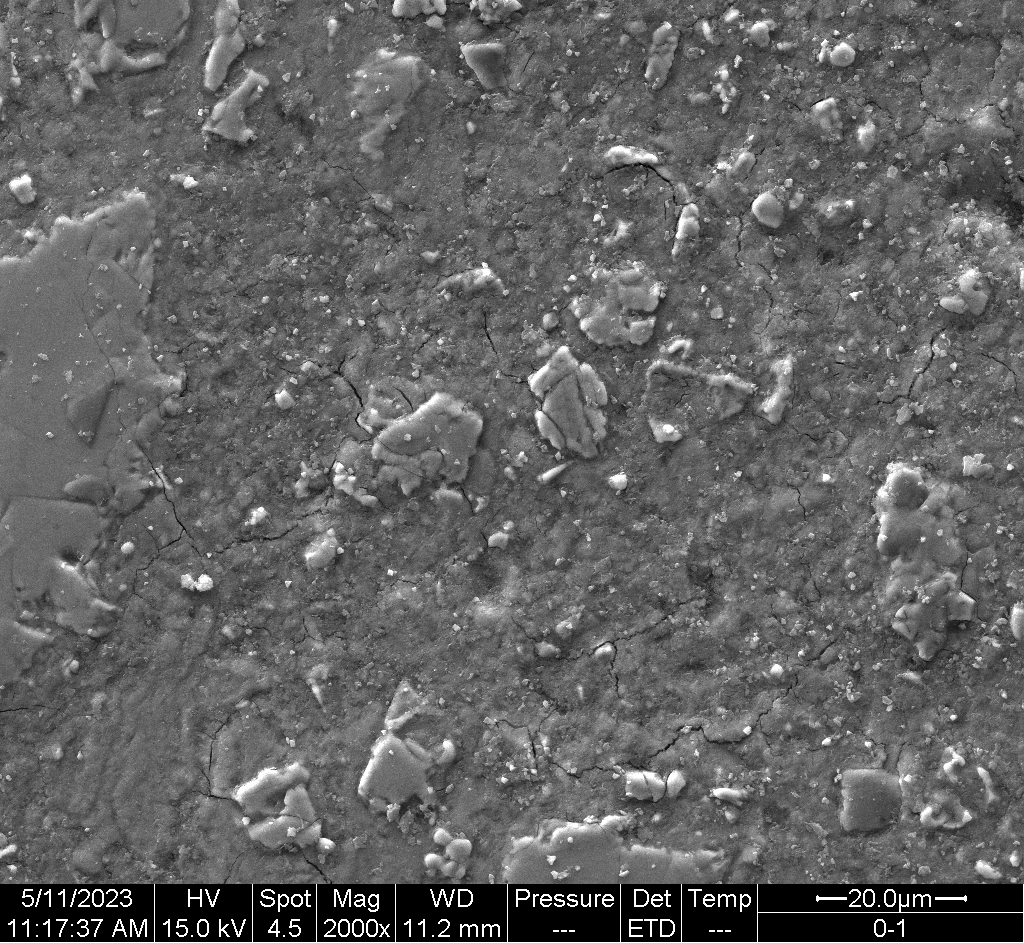
\includegraphics[height = 0.21 \linewidth]{assets/00-polished-02000x-ETD.png}} \quad
  \subcaptionbox{5000x}{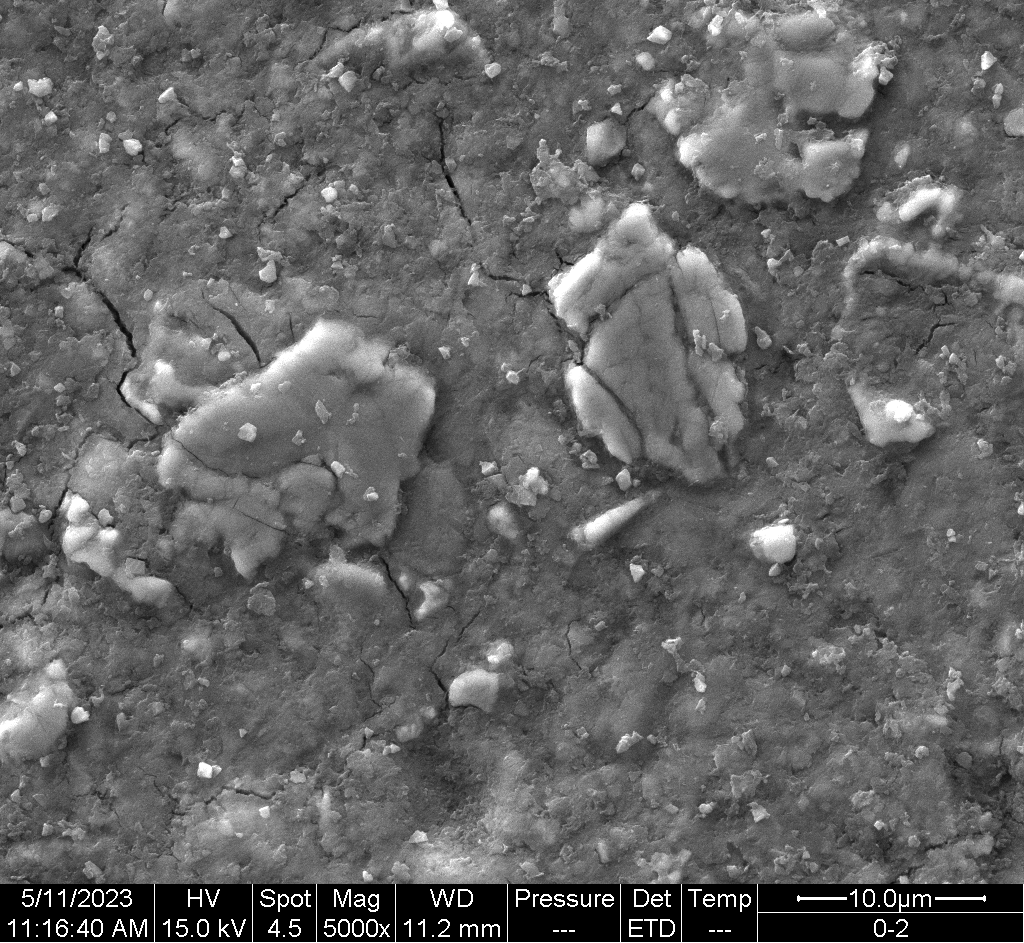
\includegraphics[height = 0.21 \linewidth]{assets/00-polished-05000x-ETD.png}} \quad
  \subcaptionbox{10000x}{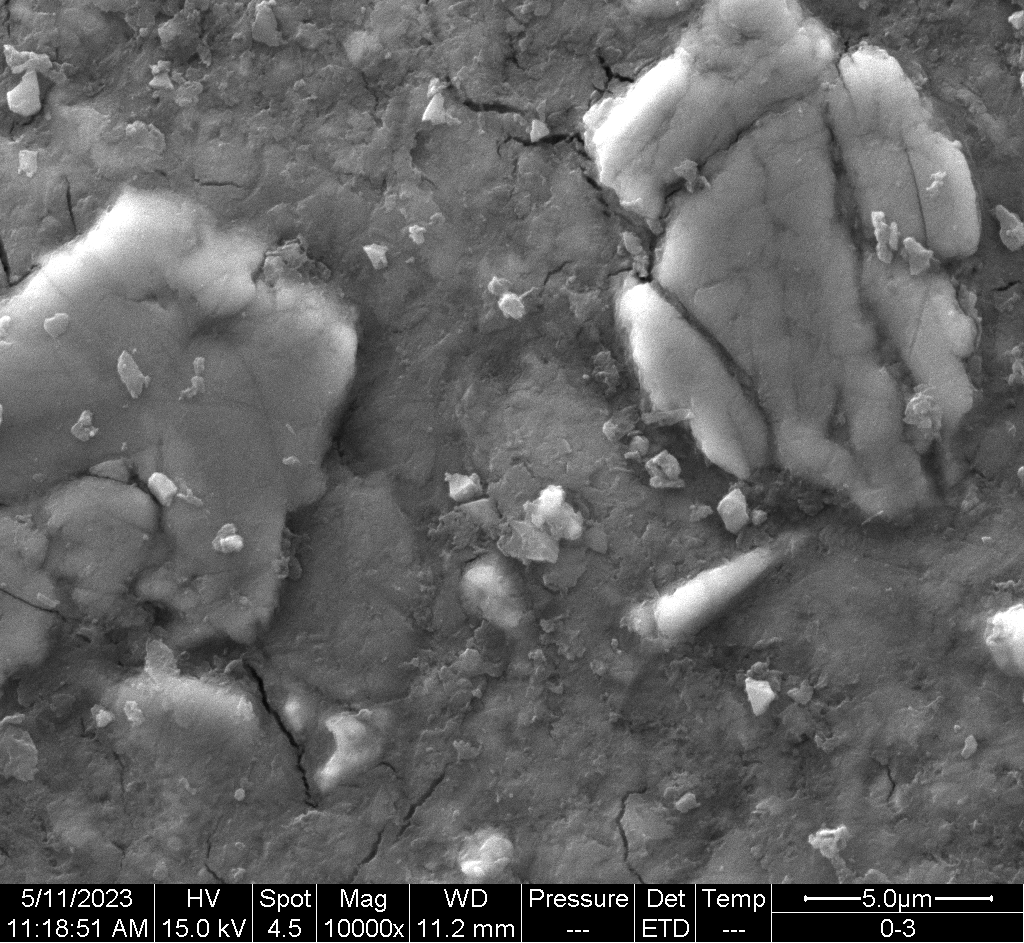
\includegraphics[height = 0.21 \linewidth]{assets/00-polished-10000x-ETD.png}}
  \caption{ETD}
\end{figure}

\begin{figure}
  \centering
  \subcaptionbox{2000x}{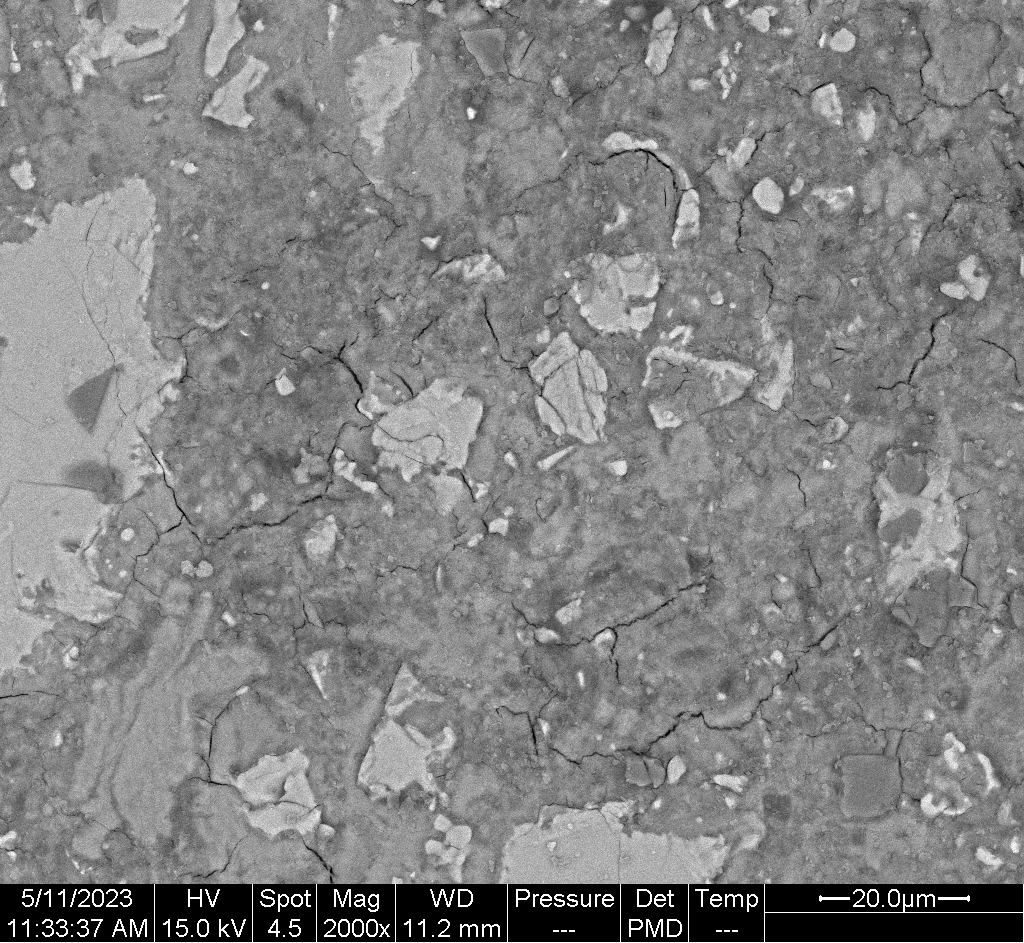
\includegraphics[height = 0.21 \linewidth]{assets/00-polished-02000x-PMD.png}} \quad
  \subcaptionbox{2500x}{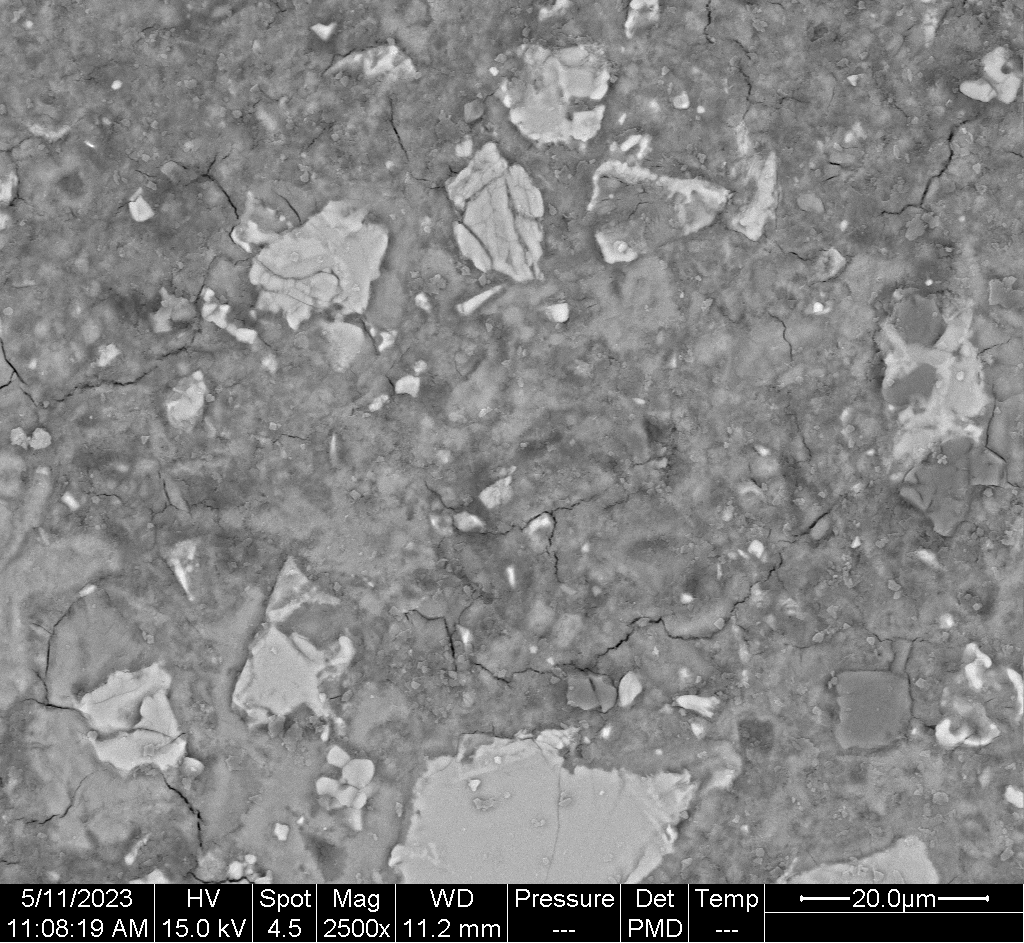
\includegraphics[height = 0.21 \linewidth]{assets/00-polished-02500x-PMD.png}} \quad
  \subcaptionbox{4788x}{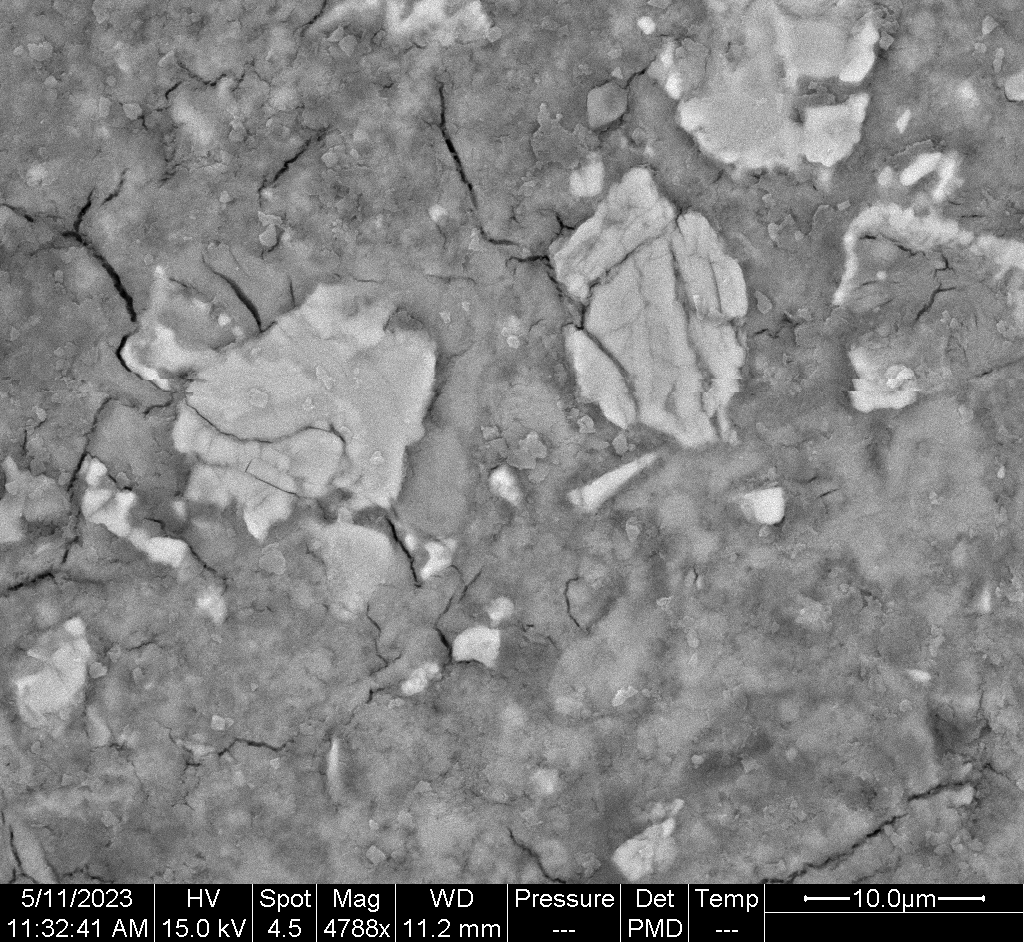
\includegraphics[height = 0.21 \linewidth]{assets/00-polished-04788x-PMD.png}} \quad
  \subcaptionbox{10000x}{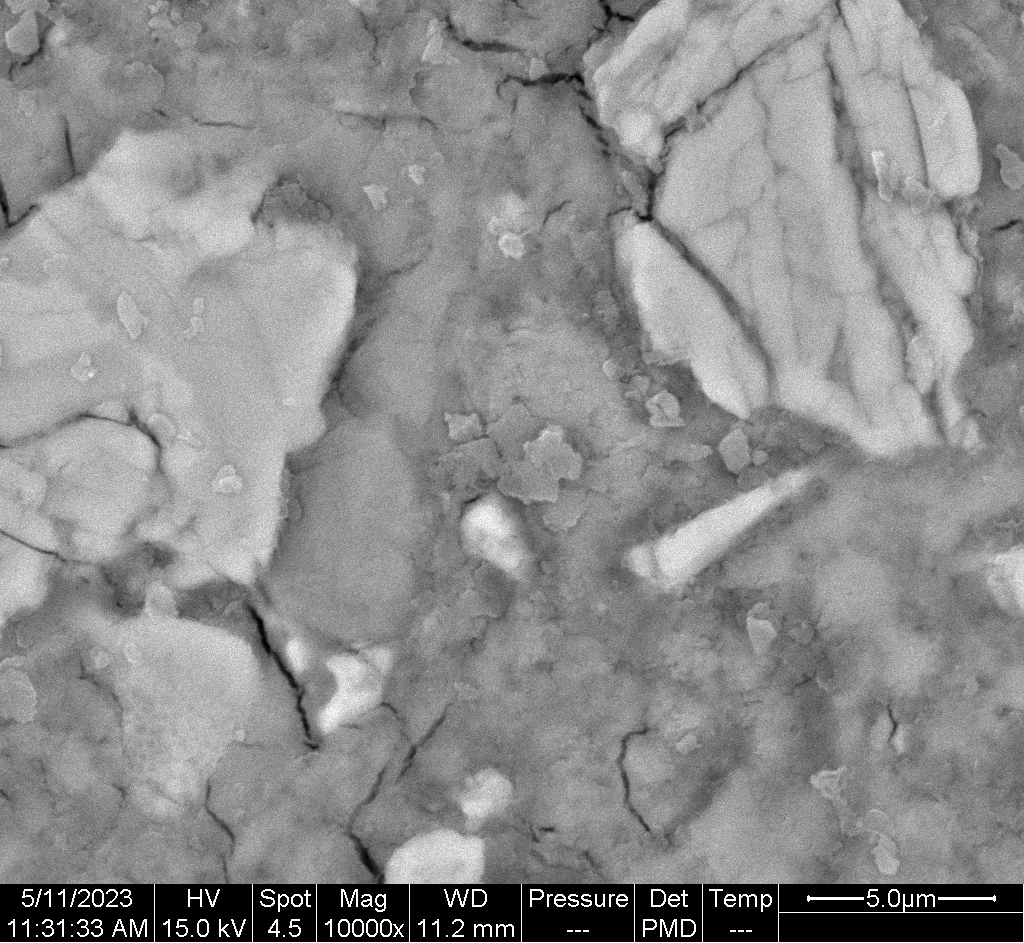
\includegraphics[height = 0.21 \linewidth]{assets/00-polished-10000x-PMD.png}}
  \caption{PMD}
\end{figure}

\subsubsection{粉煤灰: 15\%}

\begin{figure}
  \centering
  \subcaptionbox{1000x}{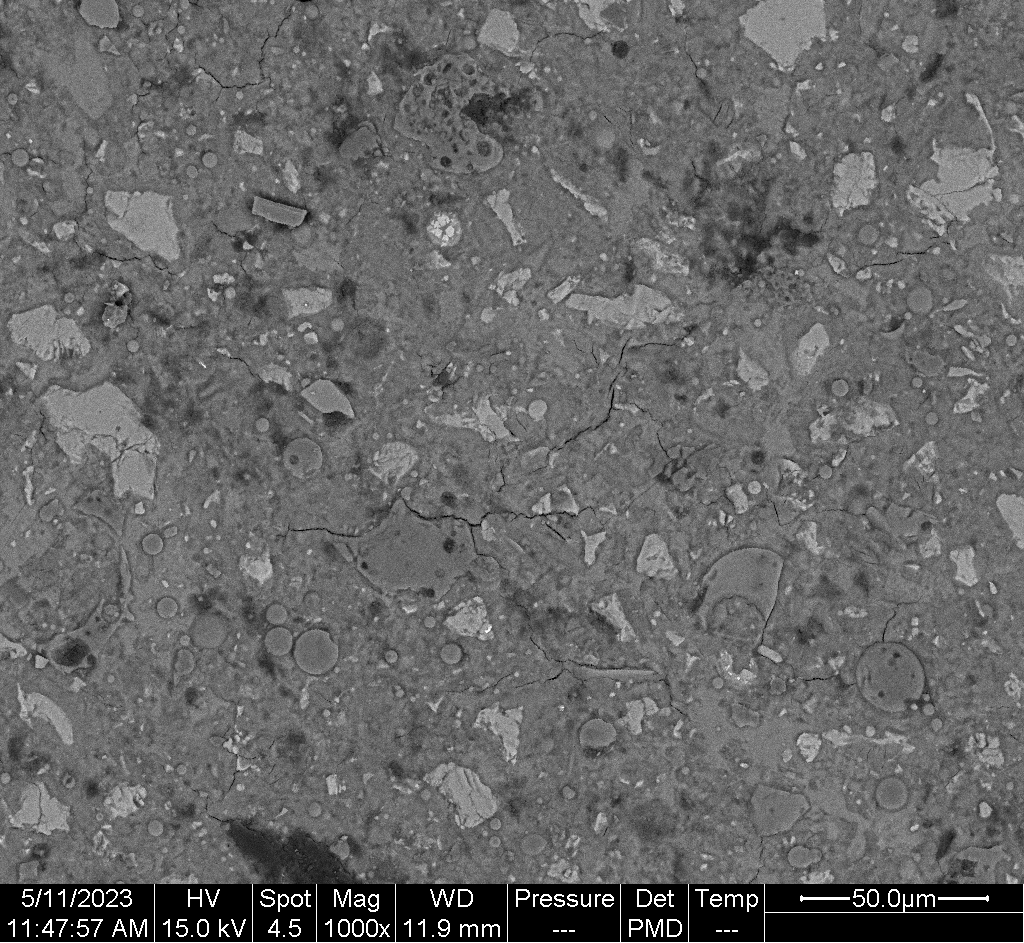
\includegraphics[height = 0.28 \linewidth]{assets/15-polished-01000x-PMD.png}} \quad
  \subcaptionbox{5000x}{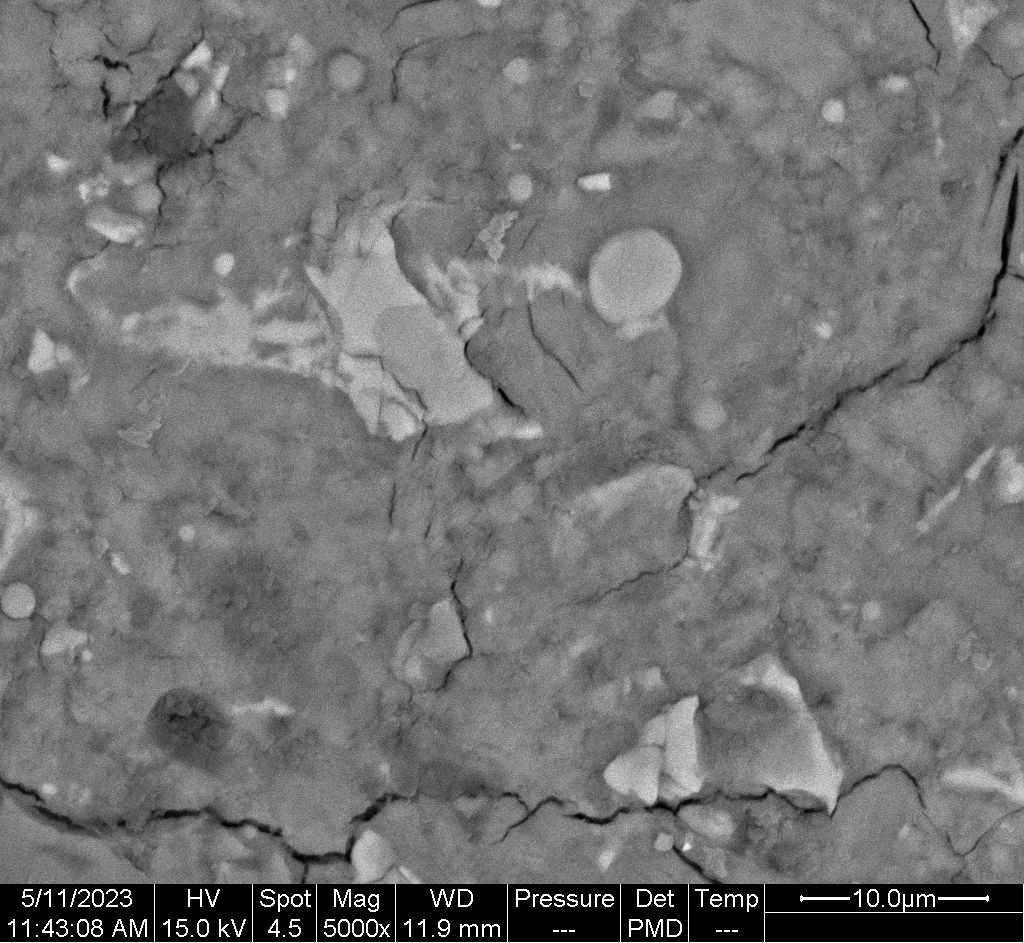
\includegraphics[height = 0.28 \linewidth]{assets/15-polished-05000x-PMD.png}} \quad
  \subcaptionbox{10000x}{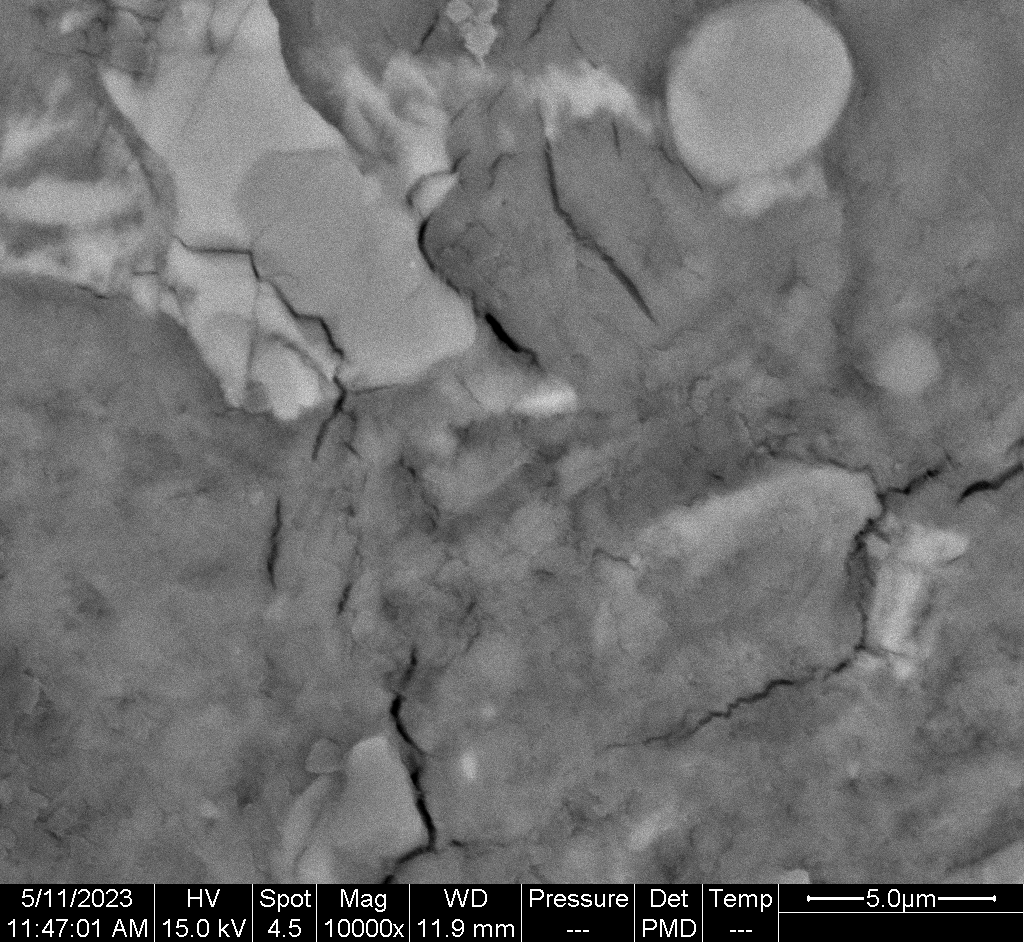
\includegraphics[height = 0.28 \linewidth]{assets/15-polished-10000x-PMD.png}}
  \caption{PMD}
\end{figure}

\subsubsection{粉煤灰: 30\%}

\begin{figure}
  \centering
  \subcaptionbox{200x}{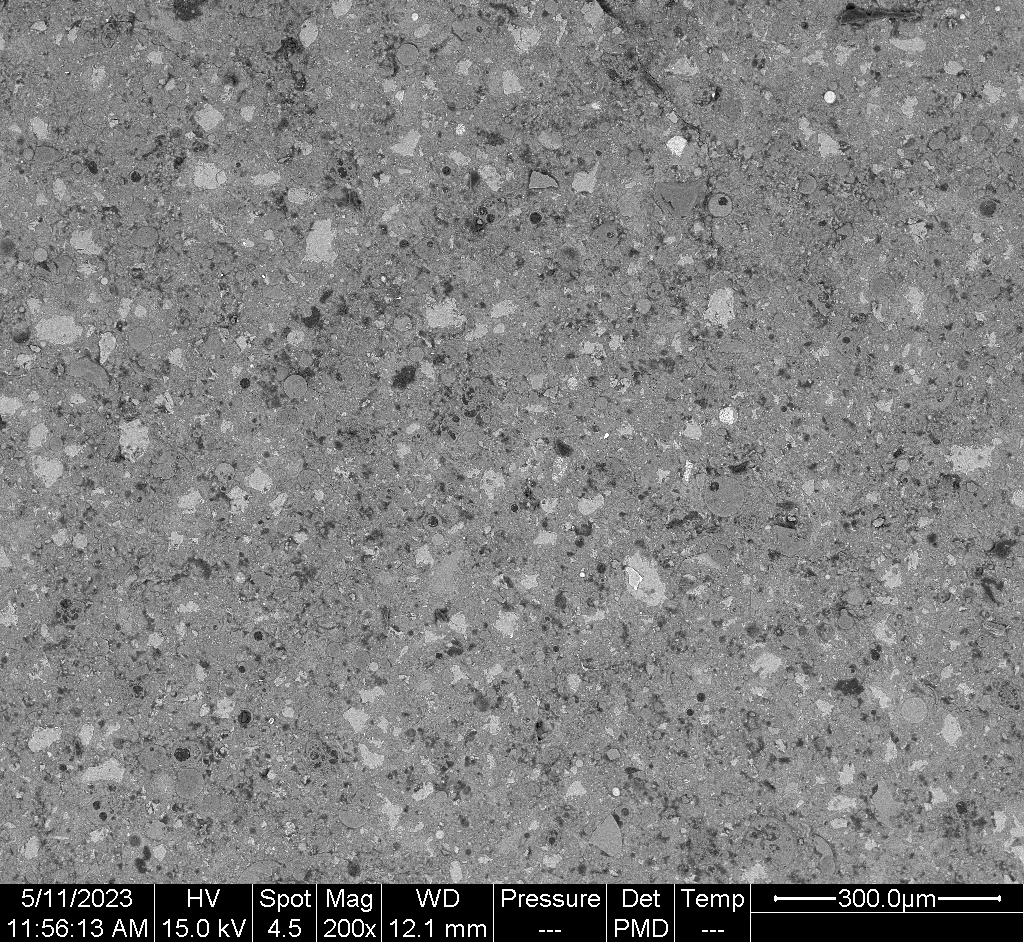
\includegraphics[height = 0.21 \linewidth]{assets/30-polished-00200x-PMD.png}} \quad
  \subcaptionbox{1000x}{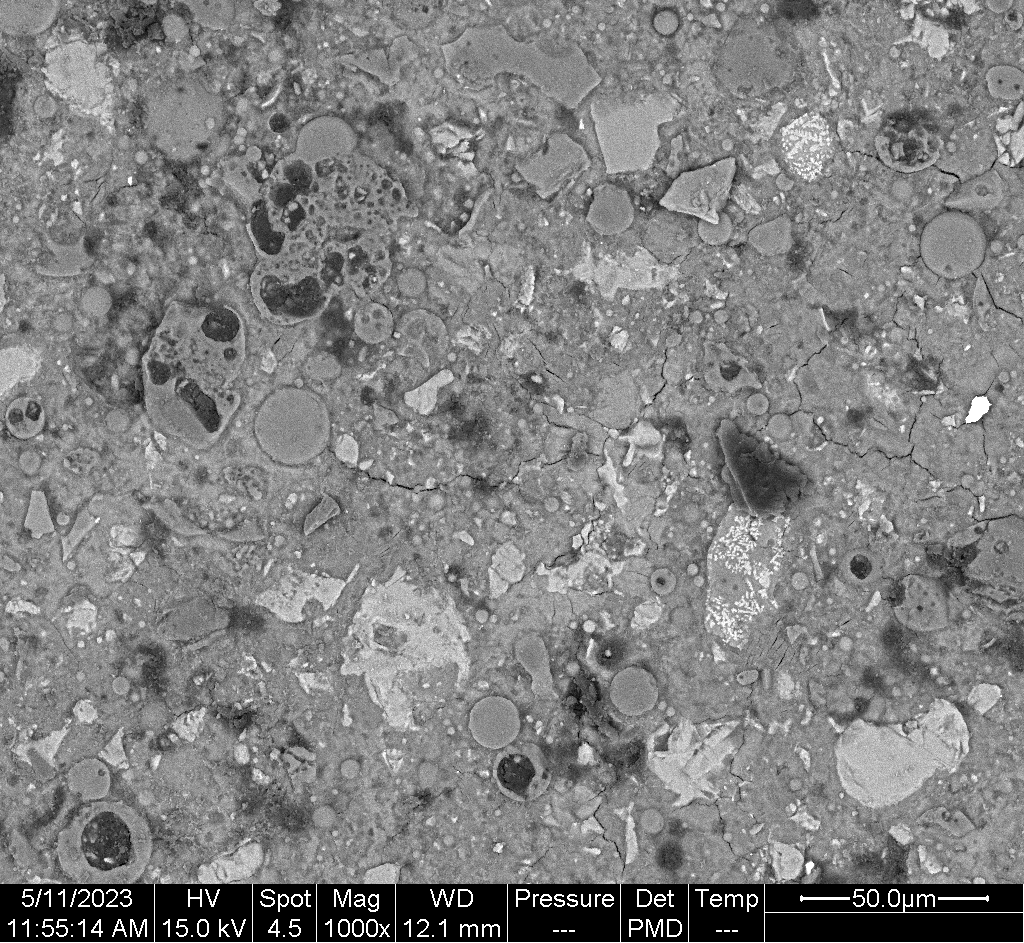
\includegraphics[height = 0.21 \linewidth]{assets/30-polished-01000x-PMD.png}} \quad
  \subcaptionbox{5000x}{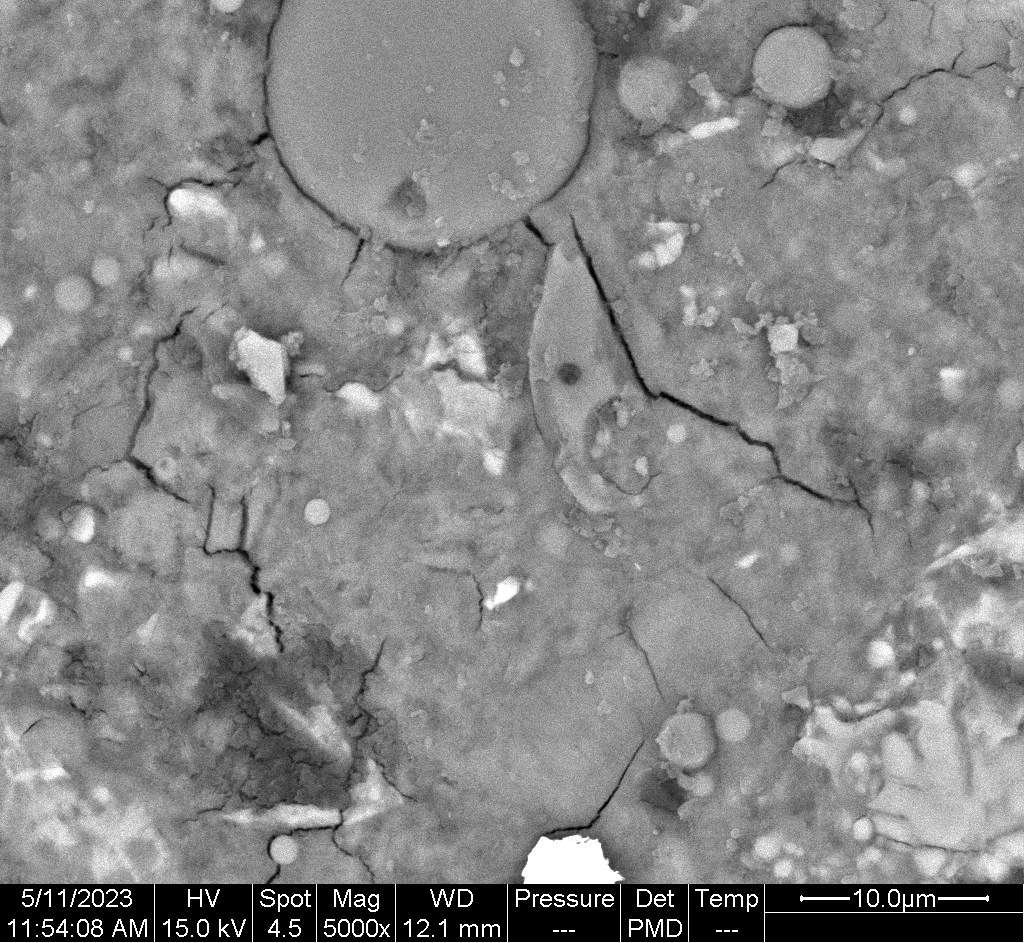
\includegraphics[height = 0.21 \linewidth]{assets/30-polished-05000x-PMD.png}} \quad
  \subcaptionbox{10000x}{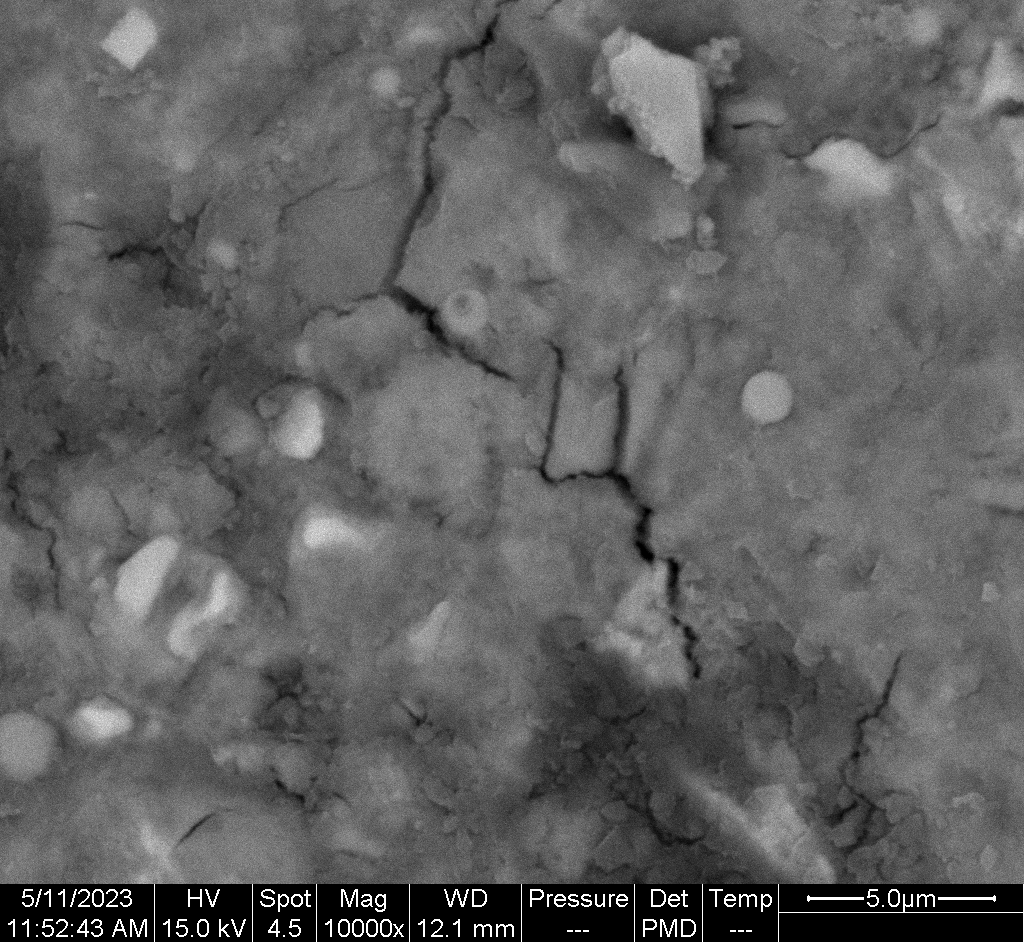
\includegraphics[height = 0.21 \linewidth]{assets/30-polished-10000x-PMD.png}}
  \caption{PMD}
\end{figure}
